% Options for packages loaded elsewhere
\PassOptionsToPackage{unicode}{hyperref}
\PassOptionsToPackage{hyphens}{url}
%
\documentclass[
]{article}
\usepackage{amsmath,amssymb}
\usepackage{iftex}
\ifPDFTeX
  \usepackage[T1]{fontenc}
  \usepackage[utf8]{inputenc}
  \usepackage{textcomp} % provide euro and other symbols
\else % if luatex or xetex
  \usepackage{unicode-math} % this also loads fontspec
  \defaultfontfeatures{Scale=MatchLowercase}
  \defaultfontfeatures[\rmfamily]{Ligatures=TeX,Scale=1}
\fi
\usepackage{lmodern}
\ifPDFTeX\else
  % xetex/luatex font selection
\fi
% Use upquote if available, for straight quotes in verbatim environments
\IfFileExists{upquote.sty}{\usepackage{upquote}}{}
\IfFileExists{microtype.sty}{% use microtype if available
  \usepackage[]{microtype}
  \UseMicrotypeSet[protrusion]{basicmath} % disable protrusion for tt fonts
}{}
\makeatletter
\@ifundefined{KOMAClassName}{% if non-KOMA class
  \IfFileExists{parskip.sty}{%
    \usepackage{parskip}
  }{% else
    \setlength{\parindent}{0pt}
    \setlength{\parskip}{6pt plus 2pt minus 1pt}}
}{% if KOMA class
  \KOMAoptions{parskip=half}}
\makeatother
\usepackage{xcolor}
\usepackage[margin=1in]{geometry}
\usepackage{color}
\usepackage{fancyvrb}
\newcommand{\VerbBar}{|}
\newcommand{\VERB}{\Verb[commandchars=\\\{\}]}
\DefineVerbatimEnvironment{Highlighting}{Verbatim}{commandchars=\\\{\}}
% Add ',fontsize=\small' for more characters per line
\usepackage{framed}
\definecolor{shadecolor}{RGB}{248,248,248}
\newenvironment{Shaded}{\begin{snugshade}}{\end{snugshade}}
\newcommand{\AlertTok}[1]{\textcolor[rgb]{0.94,0.16,0.16}{#1}}
\newcommand{\AnnotationTok}[1]{\textcolor[rgb]{0.56,0.35,0.01}{\textbf{\textit{#1}}}}
\newcommand{\AttributeTok}[1]{\textcolor[rgb]{0.13,0.29,0.53}{#1}}
\newcommand{\BaseNTok}[1]{\textcolor[rgb]{0.00,0.00,0.81}{#1}}
\newcommand{\BuiltInTok}[1]{#1}
\newcommand{\CharTok}[1]{\textcolor[rgb]{0.31,0.60,0.02}{#1}}
\newcommand{\CommentTok}[1]{\textcolor[rgb]{0.56,0.35,0.01}{\textit{#1}}}
\newcommand{\CommentVarTok}[1]{\textcolor[rgb]{0.56,0.35,0.01}{\textbf{\textit{#1}}}}
\newcommand{\ConstantTok}[1]{\textcolor[rgb]{0.56,0.35,0.01}{#1}}
\newcommand{\ControlFlowTok}[1]{\textcolor[rgb]{0.13,0.29,0.53}{\textbf{#1}}}
\newcommand{\DataTypeTok}[1]{\textcolor[rgb]{0.13,0.29,0.53}{#1}}
\newcommand{\DecValTok}[1]{\textcolor[rgb]{0.00,0.00,0.81}{#1}}
\newcommand{\DocumentationTok}[1]{\textcolor[rgb]{0.56,0.35,0.01}{\textbf{\textit{#1}}}}
\newcommand{\ErrorTok}[1]{\textcolor[rgb]{0.64,0.00,0.00}{\textbf{#1}}}
\newcommand{\ExtensionTok}[1]{#1}
\newcommand{\FloatTok}[1]{\textcolor[rgb]{0.00,0.00,0.81}{#1}}
\newcommand{\FunctionTok}[1]{\textcolor[rgb]{0.13,0.29,0.53}{\textbf{#1}}}
\newcommand{\ImportTok}[1]{#1}
\newcommand{\InformationTok}[1]{\textcolor[rgb]{0.56,0.35,0.01}{\textbf{\textit{#1}}}}
\newcommand{\KeywordTok}[1]{\textcolor[rgb]{0.13,0.29,0.53}{\textbf{#1}}}
\newcommand{\NormalTok}[1]{#1}
\newcommand{\OperatorTok}[1]{\textcolor[rgb]{0.81,0.36,0.00}{\textbf{#1}}}
\newcommand{\OtherTok}[1]{\textcolor[rgb]{0.56,0.35,0.01}{#1}}
\newcommand{\PreprocessorTok}[1]{\textcolor[rgb]{0.56,0.35,0.01}{\textit{#1}}}
\newcommand{\RegionMarkerTok}[1]{#1}
\newcommand{\SpecialCharTok}[1]{\textcolor[rgb]{0.81,0.36,0.00}{\textbf{#1}}}
\newcommand{\SpecialStringTok}[1]{\textcolor[rgb]{0.31,0.60,0.02}{#1}}
\newcommand{\StringTok}[1]{\textcolor[rgb]{0.31,0.60,0.02}{#1}}
\newcommand{\VariableTok}[1]{\textcolor[rgb]{0.00,0.00,0.00}{#1}}
\newcommand{\VerbatimStringTok}[1]{\textcolor[rgb]{0.31,0.60,0.02}{#1}}
\newcommand{\WarningTok}[1]{\textcolor[rgb]{0.56,0.35,0.01}{\textbf{\textit{#1}}}}
\usepackage{graphicx}
\makeatletter
\def\maxwidth{\ifdim\Gin@nat@width>\linewidth\linewidth\else\Gin@nat@width\fi}
\def\maxheight{\ifdim\Gin@nat@height>\textheight\textheight\else\Gin@nat@height\fi}
\makeatother
% Scale images if necessary, so that they will not overflow the page
% margins by default, and it is still possible to overwrite the defaults
% using explicit options in \includegraphics[width, height, ...]{}
\setkeys{Gin}{width=\maxwidth,height=\maxheight,keepaspectratio}
% Set default figure placement to htbp
\makeatletter
\def\fps@figure{htbp}
\makeatother
\setlength{\emergencystretch}{3em} % prevent overfull lines
\providecommand{\tightlist}{%
  \setlength{\itemsep}{0pt}\setlength{\parskip}{0pt}}
\setcounter{secnumdepth}{-\maxdimen} % remove section numbering
\ifLuaTeX
  \usepackage{selnolig}  % disable illegal ligatures
\fi
\usepackage{bookmark}
\IfFileExists{xurl.sty}{\usepackage{xurl}}{} % add URL line breaks if available
\urlstyle{same}
\hypersetup{
  pdftitle={R Part 2: Basic Data Tidying},
  pdfauthor={Emma Garlock},
  hidelinks,
  pdfcreator={LaTeX via pandoc}}

\title{R Part 2: Basic Data Tidying}
\author{Emma Garlock}
\date{June 12th, 2025}

\begin{document}
\maketitle

{
\setcounter{tocdepth}{2}
\tableofcontents
}
\section{Introduction}\label{introduction}

\begin{quote}
In this session, we are going to learn some basics about cleaning data
in R. The folder for this session is available at
\url{https://tinyurl.com/45vxsawu}.


\includegraphics{notebook_images/QR.png}

For this session you will need:

\begin{itemize}
\tightlist
\item
  FileA\_RMarkdown\_uOttawabiblio.rmd

  \begin{itemize}
  \tightlist
  \item
    \emph{This is the same notebook that I will be showing with the code
    removed}
  \item
    \emph{It's not necessary for you to use this file, you can also do
    it in a completely new notebook or R script}
  \end{itemize}
\item
  data/

  \begin{itemize}
  \tightlist
  \item
    SciHub\_SampleData.csv\\
  \item
    SciHubDOI.csv
  \end{itemize}
\end{itemize}

There are other files

\begin{itemize}
\tightlist
\item
  FileB\_MarkDown\_uOttawabiblio.rmd

  \begin{itemize}
  \tightlist
  \item
    \emph{this is the same file as above, but with the code already
    there}\\
  \end{itemize}
\item
  FileB\_MarkDown\_uOttawabiblio.nb.html

  \begin{itemize}
  \tightlist
  \item
    \emph{this is this the html file of the completed notebook}\\
  \end{itemize}
\item
  notebook\_images/

  \begin{itemize}
  \tightlist
  \item
    \emph{this is just the images that are in the notebook}
  \end{itemize}
\end{itemize}

But first we are going to have a general orientation about R Studio. If
you are going through this at a later date, you can watch
\href{https://www.youtube.com/watch?v=FIrsOBy5k58}{this} video.
\end{quote}

When you first open R you should see this:

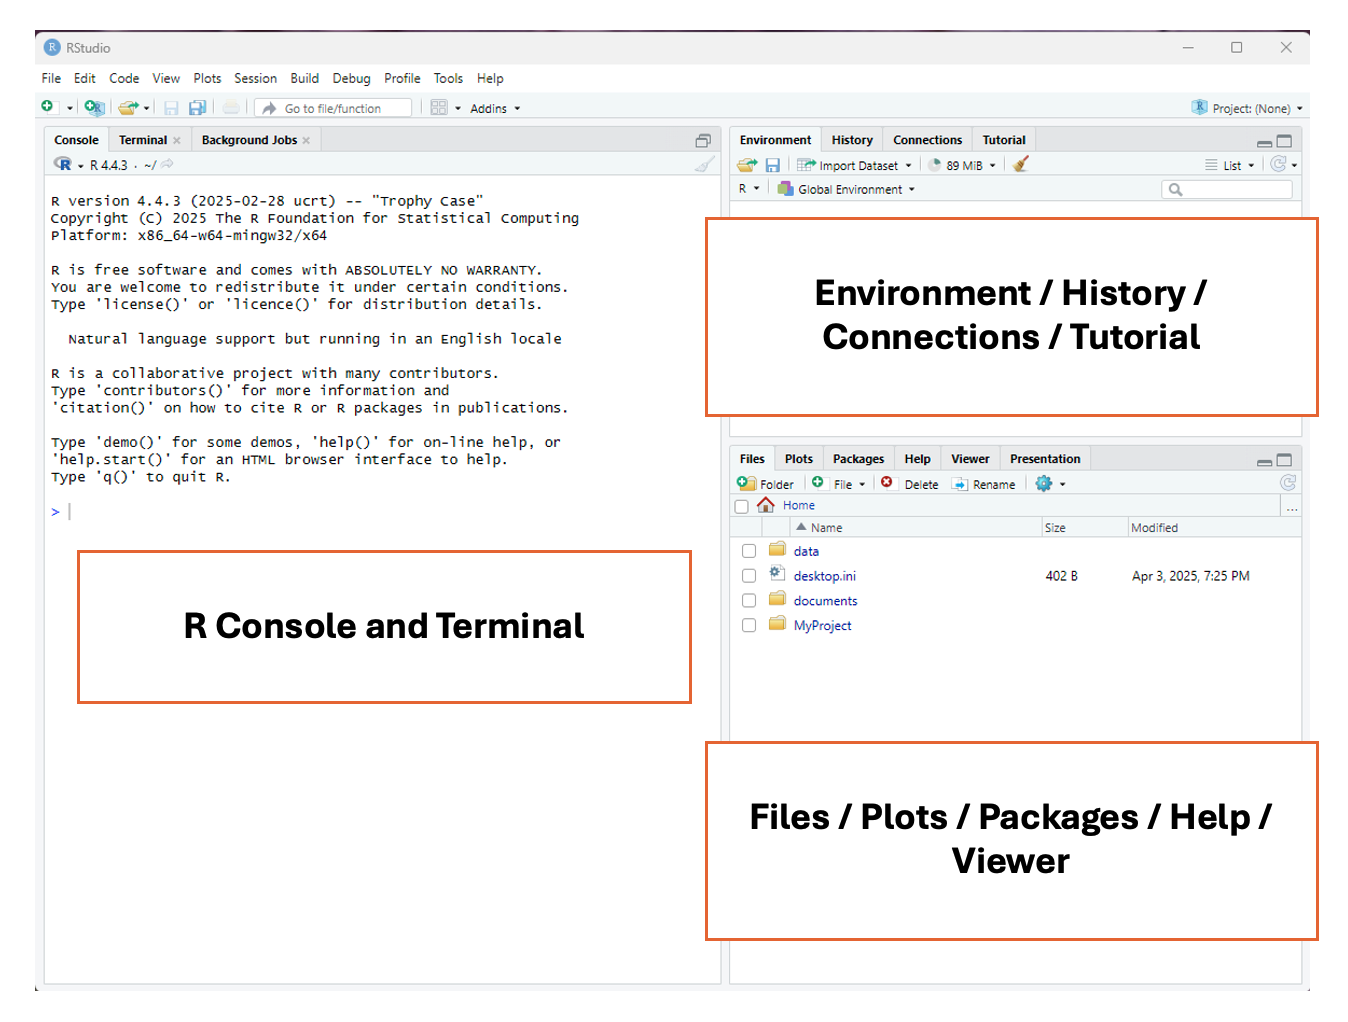
\includegraphics{notebook_images/R_panel.png} Once you open a file, you
should see this.

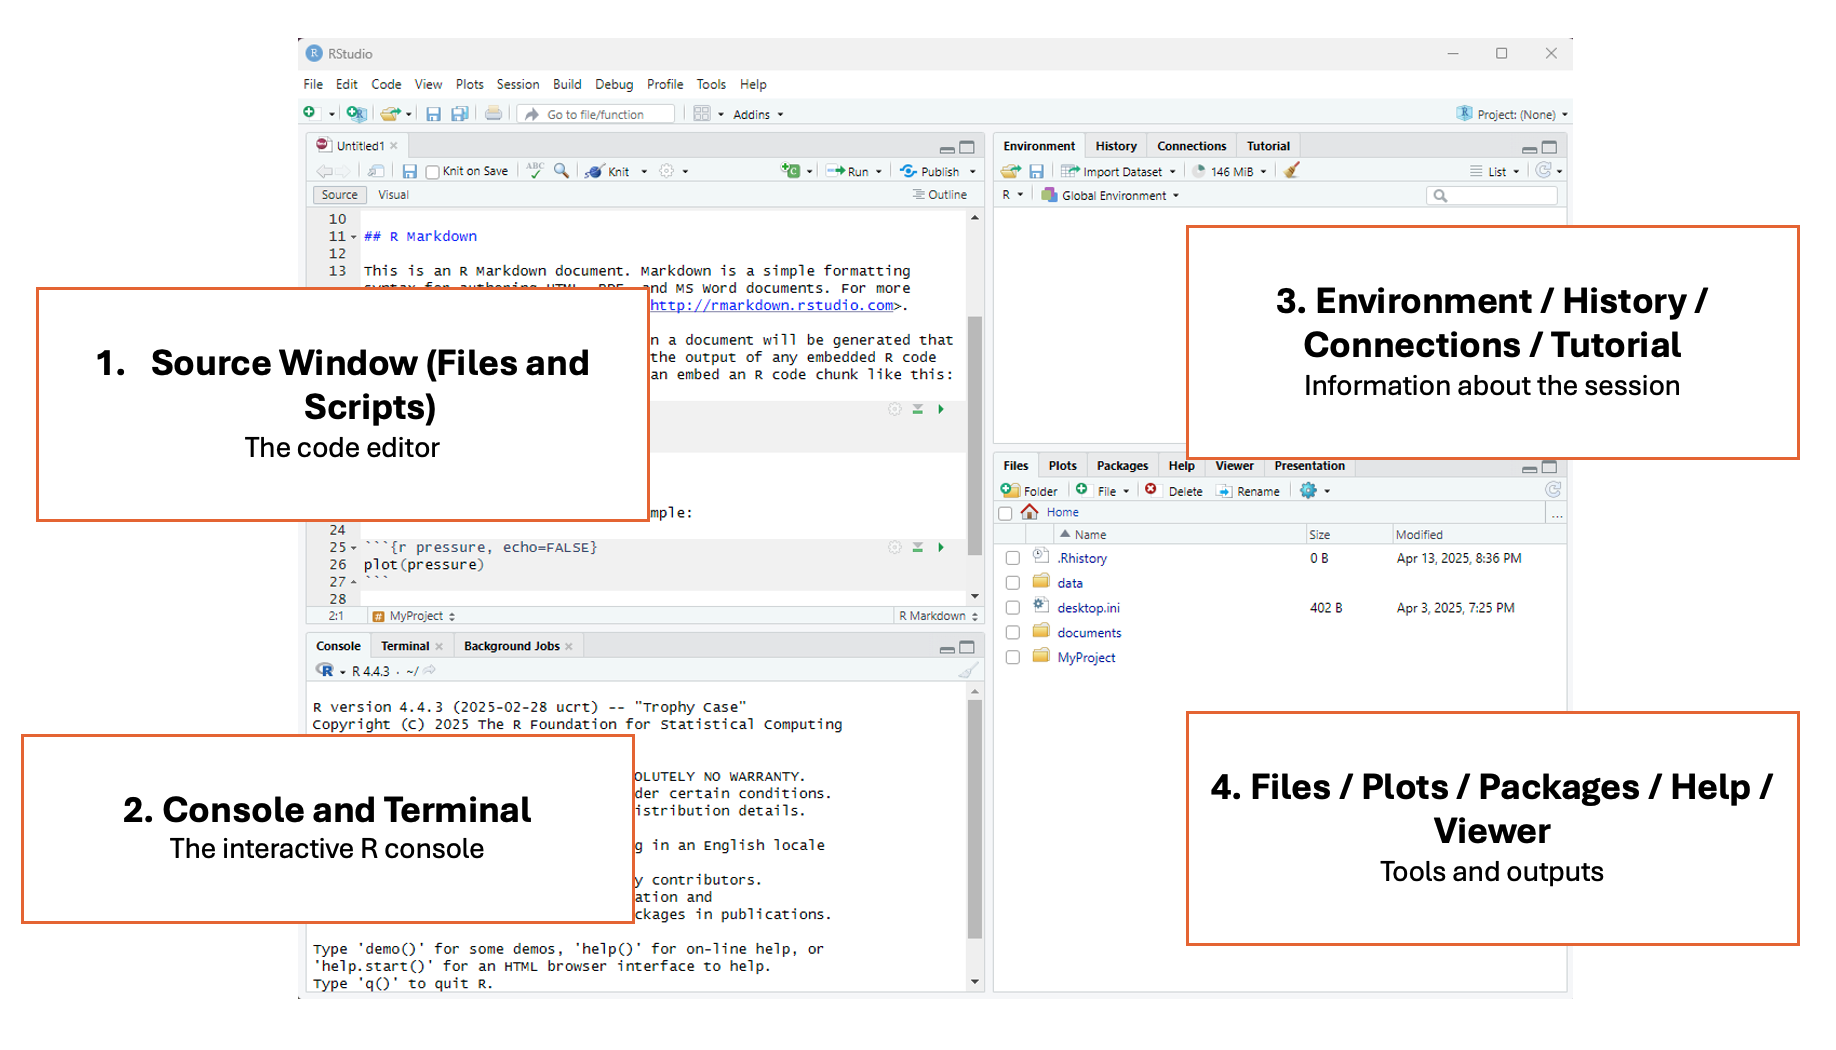
\includegraphics{notebook_images/r_4_panels.png} The above images are
from the RDM Jumpstart Program. They also have introductory lessons on
R, which are available
\href{https://alliance-rdm-gdr.github.io/rdm-jumpstart/2-ACT-1-RSetup.html}{here}.

There's 3 key features of R

\begin{enumerate}
\def\labelenumi{\arabic{enumi}.}
\tightlist
\item
  R can do operations
\end{enumerate}

\begin{Shaded}
\begin{Highlighting}[]
\DecValTok{125}\SpecialCharTok{+}\DecValTok{65}
\end{Highlighting}
\end{Shaded}

\begin{verbatim}
## [1] 190
\end{verbatim}

\begin{Shaded}
\begin{Highlighting}[]
\DecValTok{45}\SpecialCharTok{*}\DecValTok{76} 
\end{Highlighting}
\end{Shaded}

\begin{verbatim}
## [1] 3420
\end{verbatim}

\begin{Shaded}
\begin{Highlighting}[]
\DecValTok{8959}\SpecialCharTok{/}\DecValTok{32}
\end{Highlighting}
\end{Shaded}

\begin{verbatim}
## [1] 279.9688
\end{verbatim}

\begin{enumerate}
\def\labelenumi{\arabic{enumi}.}
\setcounter{enumi}{1}
\tightlist
\item
  You can assign values to objects. Then do operations on the objects
\end{enumerate}

\begin{Shaded}
\begin{Highlighting}[]
\NormalTok{x}\OtherTok{=}\DecValTok{3} 
\NormalTok{y}\OtherTok{=}\DecValTok{6}
\NormalTok{x}\SpecialCharTok{*}\NormalTok{y}
\end{Highlighting}
\end{Shaded}

\begin{verbatim}
## [1] 18
\end{verbatim}

\begin{itemize}
\tightlist
\item
  These values can be characters
\end{itemize}

\begin{Shaded}
\begin{Highlighting}[]
\NormalTok{test\_string}\OtherTok{=}\StringTok{"uOttawaBiblio"}
\FunctionTok{print}\NormalTok{(test\_string)}
\end{Highlighting}
\end{Shaded}

\begin{verbatim}
## [1] "uOttawaBiblio"
\end{verbatim}

\begin{itemize}
\tightlist
\item
  It can also be multiple values, these are what we call lists
\end{itemize}

\begin{Shaded}
\begin{Highlighting}[]
\NormalTok{test\_number\_list}\OtherTok{=}\FunctionTok{c}\NormalTok{(}\DecValTok{2}\NormalTok{,}\DecValTok{4}\NormalTok{,}\DecValTok{6}\NormalTok{,}\DecValTok{7}\NormalTok{,}\DecValTok{8}\NormalTok{,}\DecValTok{3}\NormalTok{)}
\NormalTok{test\_character\_list}\OtherTok{=}\FunctionTok{c}\NormalTok{(}\StringTok{"Spring"}\NormalTok{,}\StringTok{"Summer"}\NormalTok{,}\StringTok{"Fall"}\NormalTok{,}\StringTok{"Winter"}\NormalTok{)}
\end{Highlighting}
\end{Shaded}

\begin{itemize}
\tightlist
\item
  They can also be dataframes
\end{itemize}

\begin{Shaded}
\begin{Highlighting}[]
\NormalTok{df}\OtherTok{=}\FunctionTok{read.csv}\NormalTok{(}\StringTok{"data/testfile.csv"}\NormalTok{)}
\end{Highlighting}
\end{Shaded}

\begin{enumerate}
\def\labelenumi{\arabic{enumi}.}
\setcounter{enumi}{2}
\tightlist
\item
  R has functions, and the functions are in packages.
\end{enumerate}

We have seen a function already. \texttt{print()} and
\texttt{read.csv()} are baseR functions (aka default). The function is
the thing outside the brackets, and you perform the function on the
argument, which is inside the bracket.

So, for the example above, the function was \texttt{print()}, and the
argument was \texttt{"test\_string"}.

To get extra functions, you need to download packages. Read more about
functions and packages
\href{https://bookdown.org/nana/intror/install-and-load-packages.html}{here}.

\section{Set Up}\label{set-up}

\subsection{Working Directory}\label{working-directory}

First, we are going to set ourselves up in a working directory.

\emph{Note: if you downloaded the whole folder, and you opened one of
the provided files, ignore the advice about where to save things. It
should all be organized already}

\begin{enumerate}
\def\labelenumi{\arabic{enumi}.}
\item
  Save the R notebook or R Script file to somewhere that makes sense,
  this should be the same location where you have the data stored for
  this session. See the example below.
  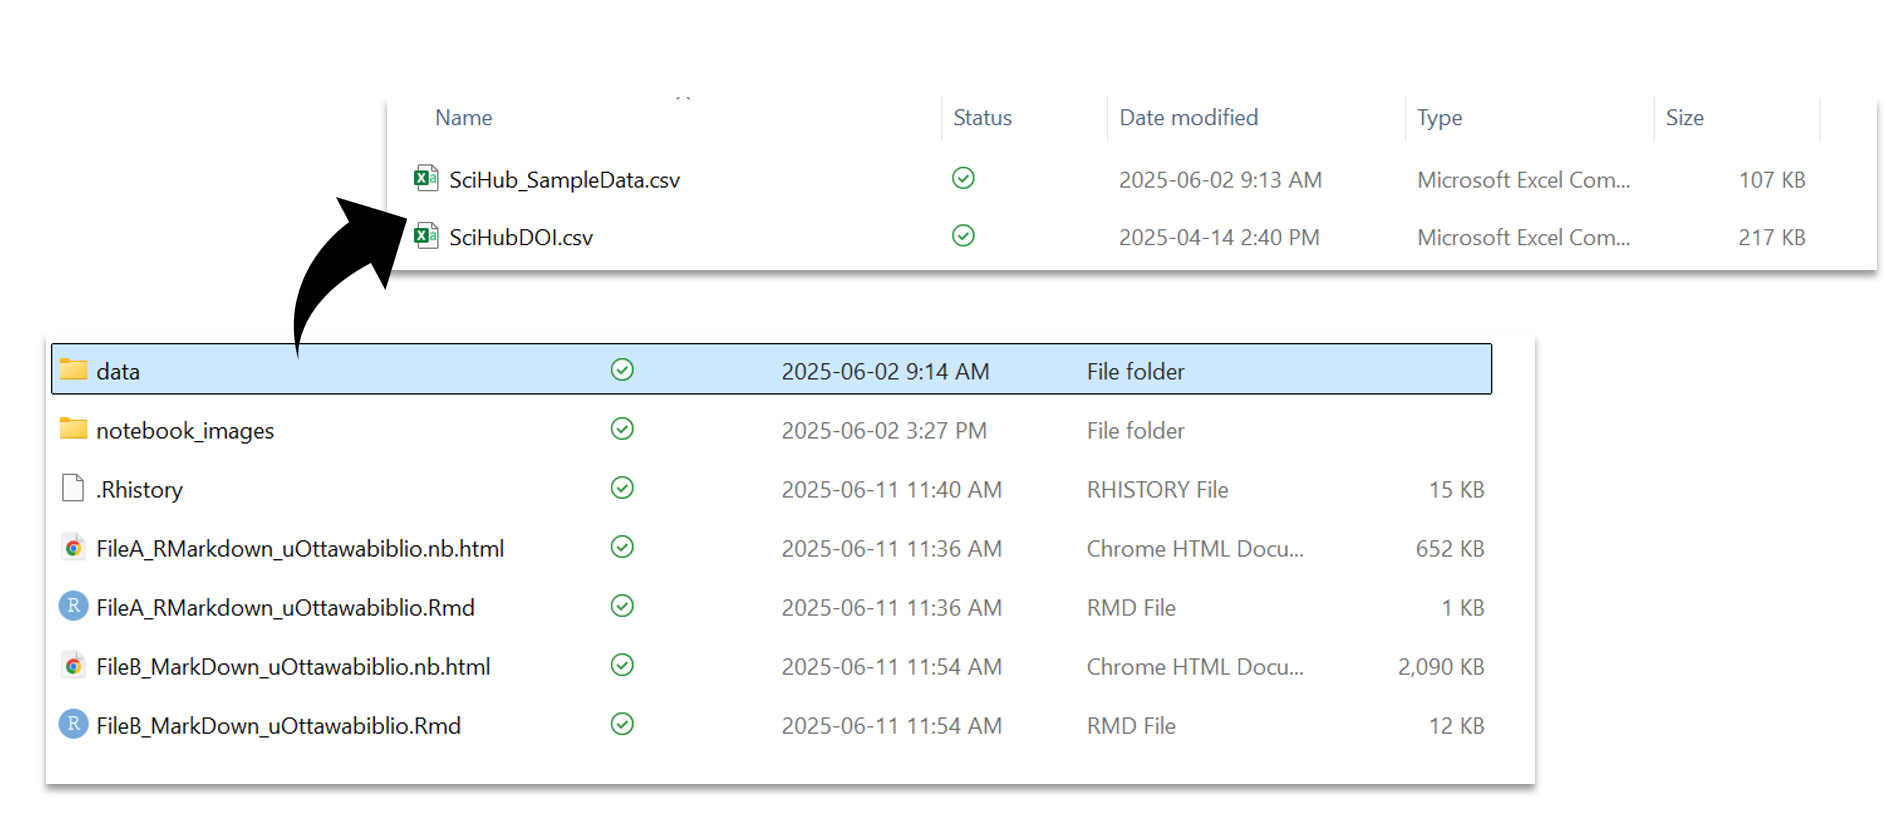
\includegraphics{notebook_images/FileSetUp.png}
\item
  Select \texttt{"Session"} from the top menu bar, then
  \texttt{"Set\ working\ directory"} then
  \texttt{"to\ Source\ file\ location"}. The directory should now be
  printed on the top of the console. See the example below.
\end{enumerate}

\subsection{Installing Tidyverse}\label{installing-tidyverse}

The following examples are going to be done using functions from
\texttt{tidyverse}. \texttt{tidyverse} is a collection of packages that
contain functions that are so commonly used for analyses, that people
decided to just makes sure that you could download these all at once AND
that they would be highly inter operable.You can learn more about
\texttt{tidyverse}
\href{https://r4ds.hadley.nz/data-transform.html}{here}

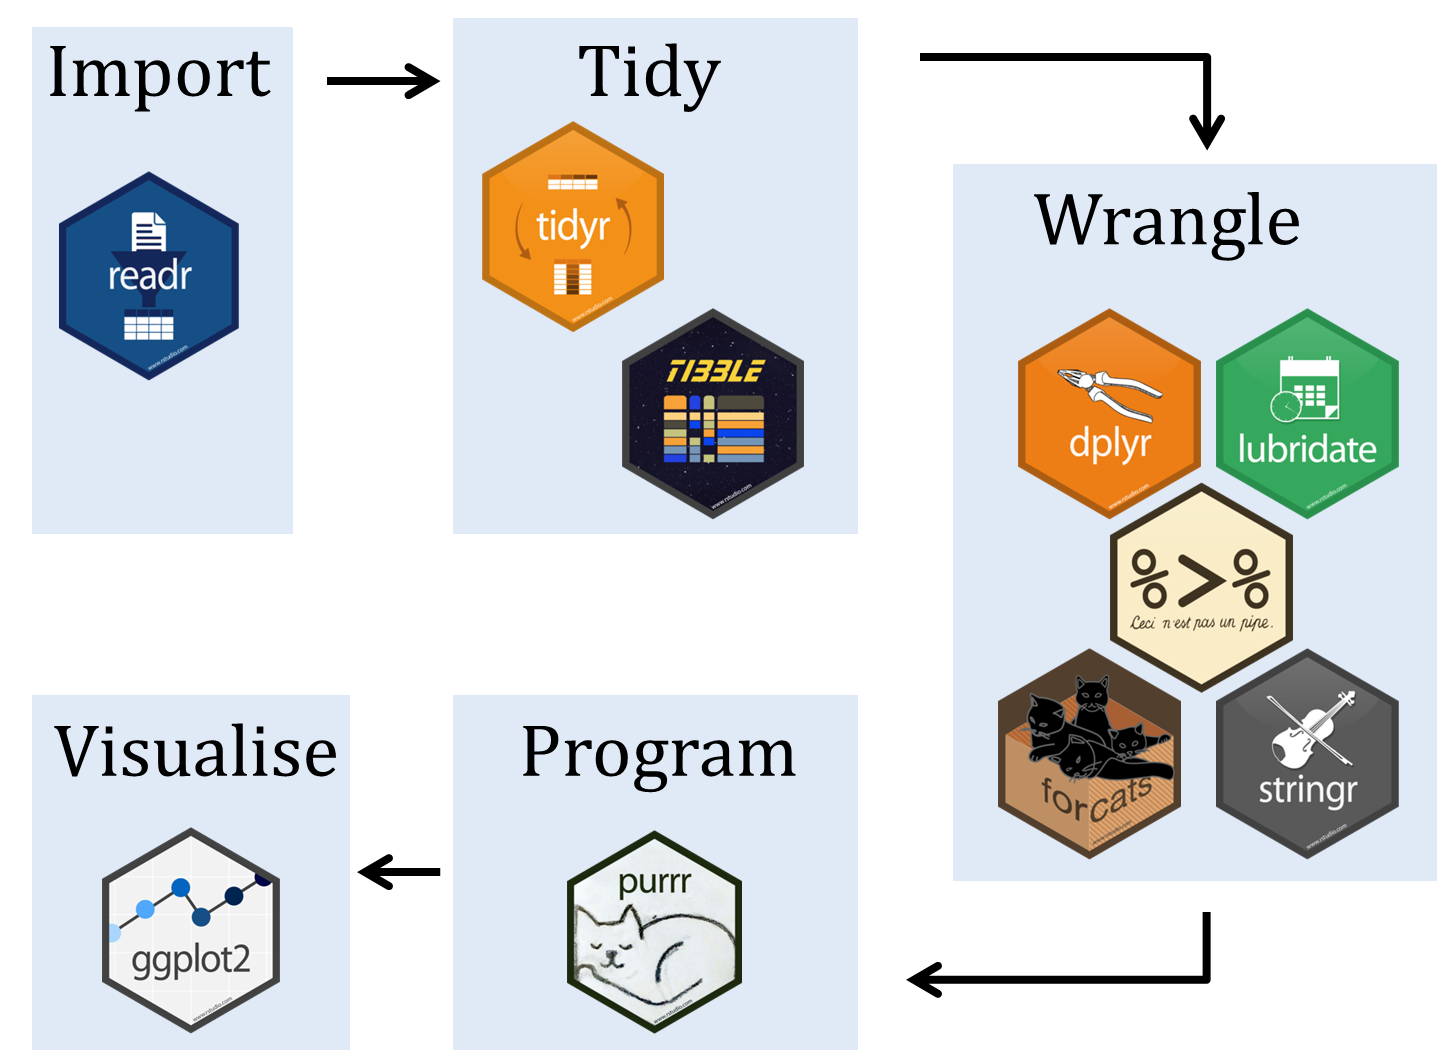
\includegraphics{notebook_images/tidy_workflow.png}

There are two ways to get a package for the first time, the first is to
run \texttt{install.packages()} with the package name in the brackets,
the second is to go over to the panel on the lower right, hit the
\texttt{"Packages"} tab, then install and type \texttt{"tidyverse"}

You do \emph{not} have to install packages every time, but you \emph{do}
need to load them every time using \texttt{library()}

Lets load our package:

\begin{Shaded}
\begin{Highlighting}[]
\CommentTok{\#this is how you install using code, this is equivalent to going through the Packages panel. I\textquotesingle{}ve commented it out since I don\textquotesingle{}t actually need to install }
\CommentTok{\#install.packages("tidyverse") }
\CommentTok{\#Loading the package}
\FunctionTok{library}\NormalTok{(tidyverse) }
\end{Highlighting}
\end{Shaded}

\begin{verbatim}
## -- Attaching core tidyverse packages ------------------------ tidyverse 2.0.0 --
## v dplyr     1.1.4     v readr     2.1.5
## v forcats   1.0.0     v stringr   1.5.1
## v ggplot2   3.5.1     v tibble    3.2.1
## v lubridate 1.9.3     v tidyr     1.3.1
## v purrr     1.0.2     
## -- Conflicts ------------------------------------------ tidyverse_conflicts() --
## x dplyr::filter() masks stats::filter()
## x dplyr::lag()    masks stats::lag()
## i Use the conflicted package (<http://conflicted.r-lib.org/>) to force all conflicts to become errors
\end{verbatim}

\subsection{Upload Data}\label{upload-data}

Now, we can load our data, and assign it the name \texttt{scihub\_df}
Then take a look at the first few rows using the \texttt{head()}
function.There is also a \texttt{tail()} function to see the last rows.
For more info on uploading data and the different formats you can use,
check out \href{https://intro2r.com/importing-data.html}{this}

I have elected to locate my data by specifying a file path. You could
also do it like \texttt{scihub\_df=read.csv(file.choose())} to open up a
file explorer.

\begin{Shaded}
\begin{Highlighting}[]
\CommentTok{\#upload the dataset, its located in the data file}
\NormalTok{scihub\_df}\OtherTok{=}\FunctionTok{read.csv}\NormalTok{(}\StringTok{"data/SciHub\_SampleData.csv"}\NormalTok{) }
\CommentTok{\#show the first 6 rows}
\FunctionTok{head}\NormalTok{(scihub\_df) }
\end{Highlighting}
\end{Shaded}

\begin{verbatim}
##             Timestamp                            DOI IP.identifier
## 1 2017-06-26 21:46:59 10.1002/14651858.CD003392.pub2       7809386
## 2 2017-09-07 22:58:24      10.1080/14786430601032386       1358764
## 3 2017-05-02 09:59:00              10.1021/la501330j       6039317
## 4 2017-07-09 09:07:20              10.1063/1.4913415       5997924
## 5 2017-05-03 08:40:56              10.1021/jp809992g        858831
## 6 2017-05-03 22:11:34              10.1021/ja025109g        858831
##   User.identifier Country.according.to.GeoIP City.according.to.GeoIP Latitude
## 1        16866302                     Canada            Boucherville 45.59137
## 2        33577860                     Canada                 Toronto 43.65323
## 3         9158745                     Canada                 Toronto 43.65323
## 4        19896736                     Canada                 Toronto 43.65323
## 5         9278539                     Canada                 Toronto 43.65323
## 6         9370108                     Canada                 Toronto 43.65323
##   Longitude
## 1 -73.43641
## 2 -79.38318
## 3 -79.38318
## 4 -79.38318
## 5 -79.38318
## 6 -79.38318
\end{verbatim}

\subsection{Rename Columns}\label{rename-columns}

Looks good, but from experience, those titles column names might make
life difficult later, lets rename them to something without spaces. We
can then check to make sure the names were changed properly and we
didn't mess anything up.

For more examples of how to rename columns check out
\href{https://sparkbyexamples.com/r-programming/rename-column-in-r/}{this}
link.

We can then use the \texttt{names()} function to see what the names of
the columns are.

\begin{Shaded}
\begin{Highlighting}[]
\CommentTok{\#change the names of scihub\_df. The list needs to be the same length as the number of columns }
\FunctionTok{colnames}\NormalTok{(scihub\_df)}\OtherTok{=}\FunctionTok{c}\NormalTok{(}\StringTok{"Timestamp"}\NormalTok{,}
                 \StringTok{"DOI"}\NormalTok{,}
                 \StringTok{"IP\_ID"}\NormalTok{,}
                 \StringTok{"User\_ID"}\NormalTok{,}
                 \StringTok{"Country\_GeoIP"}\NormalTok{,}
                 \StringTok{"City\_GeoIP"}\NormalTok{,}
                 \StringTok{"Latitude"}\NormalTok{,}
                 \StringTok{"Longitude"}\NormalTok{)}
\CommentTok{\#just print the names of columns to confirm they are the new names }
\FunctionTok{names}\NormalTok{(scihub\_df)}
\end{Highlighting}
\end{Shaded}

\begin{verbatim}
## [1] "Timestamp"     "DOI"           "IP_ID"         "User_ID"      
## [5] "Country_GeoIP" "City_GeoIP"    "Latitude"      "Longitude"
\end{verbatim}

\section{Basic Tidying and Analyses}\label{basic-tidying-and-analyses}

\subsection{Selecting Columns}\label{selecting-columns}

\texttt{tidyverse} uses something called \texttt{"pipes"}, which look
like \texttt{\%\textgreater{}\%} or \texttt{\textbar{}\textgreater{}},
which tells R to automatically use the last output as the input for the
next function. Lets see an example.

Let's say we only want a subset of the columns in \texttt{"scihub\_df",}
not all 8. We can use the \texttt{select()} function to get those

\begin{Shaded}
\begin{Highlighting}[]
\CommentTok{\#create new dataframe based on scihub\_df, just selecting the 3 columns we cant }
\NormalTok{scihub\_df\_reduced}\OtherTok{=}\NormalTok{scihub\_df}\SpecialCharTok{\%\textgreater{}\%}
  \FunctionTok{select}\NormalTok{(Timestamp,DOI,City\_GeoIP)}\CommentTok{\#just selecting these three columns }
\CommentTok{\#preview the first 6 rows so we can see if it did what we think it did }
\FunctionTok{head}\NormalTok{(scihub\_df\_reduced)}
\end{Highlighting}
\end{Shaded}

\begin{verbatim}
##             Timestamp                            DOI   City_GeoIP
## 1 2017-06-26 21:46:59 10.1002/14651858.CD003392.pub2 Boucherville
## 2 2017-09-07 22:58:24      10.1080/14786430601032386      Toronto
## 3 2017-05-02 09:59:00              10.1021/la501330j      Toronto
## 4 2017-07-09 09:07:20              10.1063/1.4913415      Toronto
## 5 2017-05-03 08:40:56              10.1021/jp809992g      Toronto
## 6 2017-05-03 22:11:34              10.1021/ja025109g      Toronto
\end{verbatim}

\subsection{Filtering Rows}\label{filtering-rows}

We could also go the other way, and only take certain rows. Let's say we
only wanted rows where the city was ``Ottawa'', we can use the
\texttt{filter()} function to find those. We can then use the
\texttt{print()} function so see our new dataframe in the console.

\emph{Note: this is case sensitive}

\begin{Shaded}
\begin{Highlighting}[]
\CommentTok{\#making a df that is just for Ottawa}
\NormalTok{scihub\_df\_ottawa}\OtherTok{=}\NormalTok{scihub\_df}\SpecialCharTok{\%\textgreater{}\%} \CommentTok{\#using the same original dataset}
  \FunctionTok{filter}\NormalTok{(City\_GeoIP}\SpecialCharTok{==}\StringTok{"Ottawa"}\NormalTok{) }\CommentTok{\#select only the rows with "Ottawa" (case sensitive) int he City\_GeoIP column}
\CommentTok{\#print the whole dataset since it\textquotesingle{}s small}
\FunctionTok{print}\NormalTok{(scihub\_df\_ottawa)}
\end{Highlighting}
\end{Shaded}

\begin{verbatim}
##             Timestamp                       DOI    IP_ID  User_ID Country_GeoIP
## 1 2017-03-26 03:00:42           10.2307/1547968  4587502  6727298        Canada
## 2 2017-07-21 16:20:54 10.1017/S1049096516001633 10172999 23057469        Canada
##   City_GeoIP Latitude Longitude
## 1     Ottawa 45.42153 -75.69719
## 2     Ottawa 45.42153 -75.69719
\end{verbatim}

\subsection{Summarizing Groups}\label{summarizing-groups}

There are a lot of basic things we can do. Lets just try getting a
summary of how many time each city appears in the dataset. We're going
to use the \texttt{"scihub\_df\_reduced"} set (the one where we used
\texttt{select()} to pick cetain columns).

We're going to start by using the \texttt{group\_by()} function. The
\texttt{group\_by()} functions creates groups based on a certain column,
and then all subsequent operations (eg. summing, averaging, counting)
are done on a \emph{per group} basis. Learn more about
\texttt{group\_by()}
\href{https://r4ds.hadley.nz/data-transform.html}{here}.

\begin{Shaded}
\begin{Highlighting}[]
\NormalTok{city\_summary}\OtherTok{=}\NormalTok{scihub\_df\_reduced}\SpecialCharTok{\%\textgreater{}\%} \CommentTok{\#using the dataset with 3 columns }
  \FunctionTok{group\_by}\NormalTok{(City\_GeoIP)}\SpecialCharTok{\%\textgreater{}\%} \CommentTok{\#make the groups based on city }
  \FunctionTok{count}\NormalTok{() }\CommentTok{\#count how many went into each group }
\CommentTok{\#see first 6 rows (they are automatically sorted alphabetically by grouping variable (aka City\_GeoIP))}
\FunctionTok{head}\NormalTok{(city\_summary)}
\end{Highlighting}
\end{Shaded}

\begin{verbatim}
## # A tibble: 6 x 2
## # Groups:   City_GeoIP [6]
##   City_GeoIP       n
##   <chr>        <int>
## 1 Ajax            12
## 2 Baddeck          2
## 3 Baie-Comeau      2
## 4 Beaconsfield    15
## 5 Boucherville    10
## 6 Bracebridge      1
\end{verbatim}

If you want to do a little sanity check, the sum of everything in column
n should be 1000.\\
We can double check like this using the \texttt{sum()} function:

\begin{Shaded}
\begin{Highlighting}[]
\FunctionTok{sum}\NormalTok{(city\_summary}\SpecialCharTok{$}\NormalTok{n)}
\end{Highlighting}
\end{Shaded}

\begin{verbatim}
## [1] 1000
\end{verbatim}

\subsection{Fixing Typos}\label{fixing-typos}

Did anyone notice anything about the summarized data?

Yes, we have two different spellings for Montréal.

Lets fix it.

We're not going to actually make a new dataset, we're just going to edit
what we already did. By adding a new line \emph{before} the
\texttt{group\_by()} where we use a function called \texttt{mutate()}.
\texttt{mutate()} is a very versatile function and can be used for a lot
of different applications. You can read more about that
\href{https://bookdown.org/yih_huynh/Guide-to-R-Book/mutate.html}{here}.

One thing you can do with \texttt{mutate()} is called a
\texttt{"nested\ function"} this is where you have a function
\emph{inside} another function. In this case we are going to use the
\texttt{replace()} function.

The \texttt{replace()} function is formatted like this:
\texttt{replace("column\ that\ we\ need\ to\ edit","what\ values\ in\ the\ column\ need\ to\ be\ edited,"What\ we\ want\ the\ new\ value\ to\ be")}

\emph{Note: there are a lot of different ways to fix typos in data sets,
this is just one of many.}

\begin{Shaded}
\begin{Highlighting}[]
\NormalTok{city\_summary}\OtherTok{=}\NormalTok{scihub\_df\_reduced}\SpecialCharTok{\%\textgreater{}\%} \CommentTok{\#3 column dataset }
  \FunctionTok{mutate}\NormalTok{(}\AttributeTok{City\_GeoIP =} \FunctionTok{replace}\NormalTok{(City\_GeoIP, City\_GeoIP }\SpecialCharTok{==} \StringTok{"Montréal"}\NormalTok{, }\StringTok{"Montreal"}\NormalTok{))}\SpecialCharTok{\%\textgreater{}\%} \CommentTok{\#fixing the error }
  \FunctionTok{group\_by}\NormalTok{(City\_GeoIP)}\SpecialCharTok{\%\textgreater{}\%}\CommentTok{\#set groups based on the city, same process as above :) }
  \FunctionTok{count}\NormalTok{()}
\end{Highlighting}
\end{Shaded}

If you remember, before we had 76 observations, now we have 75.

\subsection{Dates}\label{dates}

Notice that we have a \texttt{timestamp} column, this has both date and
the time. Could be useful, but maybe we just want the date. To do this,
we are going to load a new package, called \texttt{lubridate} which is
specifically used for working with date formats.

\begin{Shaded}
\begin{Highlighting}[]
\FunctionTok{library}\NormalTok{(lubridate) }\CommentTok{\#loading a package }
\end{Highlighting}
\end{Shaded}

We actually have a few ways we could do this.\\
1. Use \texttt{lubridate} functions\\
2. Separate using the space as a delimiter.\\
3. Extract the first 10 characters of each row into it's own column

Let's do the 1st option. We are going to do another nested function with
\texttt{mutate()} using the \texttt{ymd\_hms()} function from
\texttt{lubridate}

\begin{Shaded}
\begin{Highlighting}[]
\NormalTok{scihub\_df\_reduced\_date}\OtherTok{=}\NormalTok{scihub\_df}\SpecialCharTok{\%\textgreater{}\%} \CommentTok{\#start with the original dataset}
  \FunctionTok{select}\NormalTok{(Timestamp,DOI,City\_GeoIP)}\SpecialCharTok{\%\textgreater{}\%} \CommentTok{\#select the columns we need }
  \FunctionTok{mutate}\NormalTok{(}\AttributeTok{Timestamp=}\FunctionTok{ymd\_hms}\NormalTok{(Timestamp))}\SpecialCharTok{\%\textgreater{}\%} \CommentTok{\#make sure the time is interpreted in the correct format }
  \FunctionTok{mutate}\NormalTok{(}\AttributeTok{Date=}\FunctionTok{date}\NormalTok{(Timestamp)) }\CommentTok{\#extract the date }

\FunctionTok{head}\NormalTok{(scihub\_df\_reduced\_date) }\CommentTok{\#preview the top 6 }
\end{Highlighting}
\end{Shaded}

\begin{verbatim}
##             Timestamp                            DOI   City_GeoIP       Date
## 1 2017-06-26 21:46:59 10.1002/14651858.CD003392.pub2 Boucherville 2017-06-26
## 2 2017-09-07 22:58:24      10.1080/14786430601032386      Toronto 2017-09-07
## 3 2017-05-02 09:59:00              10.1021/la501330j      Toronto 2017-05-02
## 4 2017-07-09 09:07:20              10.1063/1.4913415      Toronto 2017-07-09
## 5 2017-05-03 08:40:56              10.1021/jp809992g      Toronto 2017-05-03
## 6 2017-05-03 22:11:34              10.1021/ja025109g      Toronto 2017-05-03
\end{verbatim}

\subsection{The Separate function}\label{the-separate-function}

Lets try it using the \texttt{separate()} function to get the time
(Option 2)

\begin{Shaded}
\begin{Highlighting}[]
\NormalTok{scihub\_df\_reduced\_time}\OtherTok{=}\NormalTok{scihub\_df}\SpecialCharTok{\%\textgreater{}\%} \CommentTok{\#same selection procedure as above }
  \FunctionTok{select}\NormalTok{(Timestamp,DOI,City\_GeoIP)}\SpecialCharTok{\%\textgreater{}\%}
  \FunctionTok{separate}\NormalTok{(Timestamp, }\FunctionTok{c}\NormalTok{(}\StringTok{"Date"}\NormalTok{, }\StringTok{"Time"}\NormalTok{), }\StringTok{" "}\NormalTok{) }\CommentTok{\#separate the date and time based on the space (the blank in between the quotes) and call the two new columns "Date" and "time" }

\FunctionTok{head}\NormalTok{(scihub\_df\_reduced\_time)}
\end{Highlighting}
\end{Shaded}

\begin{verbatim}
##         Date     Time                            DOI   City_GeoIP
## 1 2017-06-26 21:46:59 10.1002/14651858.CD003392.pub2 Boucherville
## 2 2017-09-07 22:58:24      10.1080/14786430601032386      Toronto
## 3 2017-05-02 09:59:00              10.1021/la501330j      Toronto
## 4 2017-07-09 09:07:20              10.1063/1.4913415      Toronto
## 5 2017-05-03 08:40:56              10.1021/jp809992g      Toronto
## 6 2017-05-03 22:11:34              10.1021/ja025109g      Toronto
\end{verbatim}

There is also a \texttt{paste()} function in R. It's very similar to the
concatenate in Excel, and you can learn more about it
\href{https://www.digitalocean.com/community/tutorials/paste-in-r}{here}.

Finally, you will probably want to save your work after everything. To
do this, we can use the \texttt{write.csv()} function.

The format for this is \texttt{write.csv(data,\ filepath)}. After
running this, you can check the file location to see if a new file has
appeared.

\begin{Shaded}
\begin{Highlighting}[]
\FunctionTok{write.csv}\NormalTok{(scihub\_df\_reduced,}\StringTok{"data/scihub\_df\_reduced.csv"}\NormalTok{)}
\end{Highlighting}
\end{Shaded}

\section{Bonus Content if we get
time}\label{bonus-content-if-we-get-time}

\subsection{Joins}\label{joins}

So, we have this information about DOI, but what if we want more
information? Luckily we have the title and other publication information
available from Zotero, and we can export a csv from Zotero and ``join''
it to our existing dataset.

This csv is going to have a lot of columns. But maybe we only want DOI
(Column 9), Title (Column 5) and Publication Year (Column 3). Before
when we selected, we used the names of the columns, but we can also
select based on the column number.

Notice that we were able to pipe the \texttt{read.csv} immediately into
the \texttt{select()}

\begin{Shaded}
\begin{Highlighting}[]
\NormalTok{zotero}\OtherTok{=}\FunctionTok{read.csv}\NormalTok{(}\StringTok{"data/SciHubDOI.csv"}\NormalTok{)}\SpecialCharTok{\%\textgreater{}\%}
  \FunctionTok{select}\NormalTok{(}\DecValTok{9}\NormalTok{,}\DecValTok{5}\NormalTok{,}\DecValTok{3}\NormalTok{) }\CommentTok{\#selecting based on position rather than name }
\FunctionTok{head}\NormalTok{(zotero)}
\end{Highlighting}
\end{Shaded}

\begin{verbatim}
##                       DOI
## 1       10.1021/jp809992g
## 2   10.1093/beheco/arx008
## 3       10.1149/1.2069301
## 4       10.1002/dap.30253
## 5 10.1126/science.aaa9092
## 6  10.1002/anie.201605430
##                                                                                                               Title
## 1 Spectroscopic Studies of Pristine and Fluorinated Nano-ZrO<sub>2</sub> in Photostimulated Heterogeneous Processes
## 2                                                                           Why is the giant panda black and white?
## 3    Solid‐State NMR Studies of Ions in Protective Coatings: II . Lithium and Cesium Ions in Polybutadiene Coatings
## 4                                                      How to learn and use your institution's student voting rates
## 5                                                                            Boreal forest health and global change
## 6                                   From Alkanes to Carboxylic Acids: Terminal Oxygenation by a Fungal Peroxygenase
##   Publication.Year
## 1             2009
## 2             2017
## 3             1992
## 4             2016
## 5             2015
## 6             2016
\end{verbatim}

Now, lets join the datasets together. We are using \texttt{left\_join()}
here, but there are lots of different types of joins that you can learn
more about
\href{https://r4ds.hadley.nz/joins.html\#sec-mutating-joins}{here}.

\begin{Shaded}
\begin{Highlighting}[]
\NormalTok{scihub\_zotero}\OtherTok{=}\NormalTok{scihub\_df\_reduced}\SpecialCharTok{\%\textgreater{}\%}
  \FunctionTok{left\_join}\NormalTok{(zotero,}\AttributeTok{by=}\StringTok{"DOI"}\NormalTok{) }\CommentTok{\#telling it to join the dataset zotero by the values in column DOI }

\FunctionTok{head}\NormalTok{(scihub\_zotero)}
\end{Highlighting}
\end{Shaded}

\begin{verbatim}
##             Timestamp                            DOI   City_GeoIP
## 1 2017-06-26 21:46:59 10.1002/14651858.CD003392.pub2 Boucherville
## 2 2017-09-07 22:58:24      10.1080/14786430601032386      Toronto
## 3 2017-05-02 09:59:00              10.1021/la501330j      Toronto
## 4 2017-07-09 09:07:20              10.1063/1.4913415      Toronto
## 5 2017-05-03 08:40:56              10.1021/jp809992g      Toronto
## 6 2017-05-03 22:11:34              10.1021/ja025109g      Toronto
##                                                                                                                                                                              Title
## 1                                                                                                                 Breast stimulation for cervical ripening and induction of labour
## 2                                                                                                         Adsorption characteristics of parent and copper-sputtered RD silica gels
## 3 Micropatterned Ferrocenyl Monolayers Covalently Bound to Hydrogen-Terminated Silicon Surfaces: Effects of Pattern Size on the Cyclic Voltammetry and Capacitance Characteristics
## 4                                                                              Conduction of molecular electronic devices: Qualitative insights through atom-atom polarizabilities
## 5                                                                Spectroscopic Studies of Pristine and Fluorinated Nano-ZrO<sub>2</sub> in Photostimulated Heterogeneous Processes
## 6                                Structural Basis for BABIM Inhibition of Botulinum Neurotoxin Type B Protease [ <i>J. Am. Chem. Soc.</i> <b>2000</b> , <i>122</i> , 11268−11269].
##   Publication.Year
## 1             2005
## 2             2007
## 3             2014
## 4             2015
## 5             2009
## 6             2002
\end{verbatim}

\subsection{Pivots}\label{pivots}

We're going to combine a few things we have seen so far. 1. making
lists.\\
2. \texttt{group\_by()}, but this time we will have TWO groupings.\\
3. \texttt{filter}, but this time with a list of options and not just
one.

We're going to start with our reduced set. Let's refresh on what it
looks like.

\begin{Shaded}
\begin{Highlighting}[]
\FunctionTok{head}\NormalTok{(scihub\_df\_reduced)}
\end{Highlighting}
\end{Shaded}

\begin{verbatim}
##             Timestamp                            DOI   City_GeoIP
## 1 2017-06-26 21:46:59 10.1002/14651858.CD003392.pub2 Boucherville
## 2 2017-09-07 22:58:24      10.1080/14786430601032386      Toronto
## 3 2017-05-02 09:59:00              10.1021/la501330j      Toronto
## 4 2017-07-09 09:07:20              10.1063/1.4913415      Toronto
## 5 2017-05-03 08:40:56              10.1021/jp809992g      Toronto
## 6 2017-05-03 22:11:34              10.1021/ja025109g      Toronto
\end{verbatim}

We have 3 columns: Timestamp, DOI and City\_GeoIP. But maybe we want to
see how often each DOI comes up in each city and the organize the
information so we have 1 column for each city.

For the sake of not creating a huge dataset, we're going to only include
certain cities. Lets define those using a list.

\begin{Shaded}
\begin{Highlighting}[]
\NormalTok{cities\_list}\OtherTok{=}\FunctionTok{c}\NormalTok{(}\StringTok{"Ottawa"}\NormalTok{,}\StringTok{"Toronto"}\NormalTok{,}\StringTok{"Montreal"}\NormalTok{,}\StringTok{"Burnaby"}\NormalTok{)}
\end{Highlighting}
\end{Shaded}

Now we know what we're working with, we can string everything together.
The final line is \texttt{pivot\_wider}, it will be easier to explain
what it does after you have seen the final product.

\begin{Shaded}
\begin{Highlighting}[]
\NormalTok{scihub\_pivot}\OtherTok{=}\NormalTok{scihub\_df\_reduced}\SpecialCharTok{\%\textgreater{}\%}
  \FunctionTok{group\_by}\NormalTok{(City\_GeoIP,DOI)}\SpecialCharTok{\%\textgreater{}\%} \CommentTok{\#group by city and DOI, so we\textquotesingle{}ll get a summary of the doi count per city }
  \FunctionTok{count}\NormalTok{()}\SpecialCharTok{\%\textgreater{}\%}
  \FunctionTok{filter}\NormalTok{(City\_GeoIP }\SpecialCharTok{\%in\%}\NormalTok{ cities\_list)}\SpecialCharTok{\%\textgreater{}\%} \CommentTok{\#filter, but only keep values that appear in cities\_list}
  \FunctionTok{pivot\_wider}\NormalTok{(}\AttributeTok{id\_cols=}\NormalTok{DOI,}\AttributeTok{names\_from=}\NormalTok{City\_GeoIP,}\AttributeTok{values\_from=}\NormalTok{n)}\CommentTok{\#here is the pivot, we say that the rows should be based on DOI, the new column names are going to be the city, and the values in the cells are the counts of that DOI in that city}

\FunctionTok{head}\NormalTok{(scihub\_pivot)}
\end{Highlighting}
\end{Shaded}

\begin{verbatim}
## # A tibble: 6 x 5
## # Groups:   DOI [6]
##   DOI                           Burnaby Montreal Ottawa Toronto
##   <chr>                           <int>    <int>  <int>   <int>
## 1 10.1021/jp011934s                   1       NA     NA       1
## 2 10.1126/science.197.4307.967        1       NA     NA       3
## 3 10.1002/wcc.81                     NA        2     NA       4
## 4 10.1016/0006-8993(77)90423-1       NA        1     NA      NA
## 5 10.1016/S2214-109X(16)30188-7      NA        3     NA      NA
## 6 10.1037/a0017364                   NA        1     NA      NA
\end{verbatim}

\end{document}
